\chapter{System Architecture \& Code Structure}
\label{ch:architecture}

This chapter outlines the high-level architecture of the password manager and explains how the project is organized into modular components.



\section{Cryptographic Pipeline}
The system uses a robust cryptographic pipeline for both encryption and decryption. The core principle is the \textbf{Encrypt-then-MAC} construction, which has been proven to be generically secure for authenticated encryption \cite{bellare2000, krawczyk2001}.

\subsection{Encryption Pipeline}
As illustrated in Figure \ref{fig:enc_flow}, the process starts with a Master Password and a random Salt. These are fed into PBKDF2 to derive a Master Key, which is then split into an AES Key and an HMAC Key.

\begin{figure}[h]
    \centering
    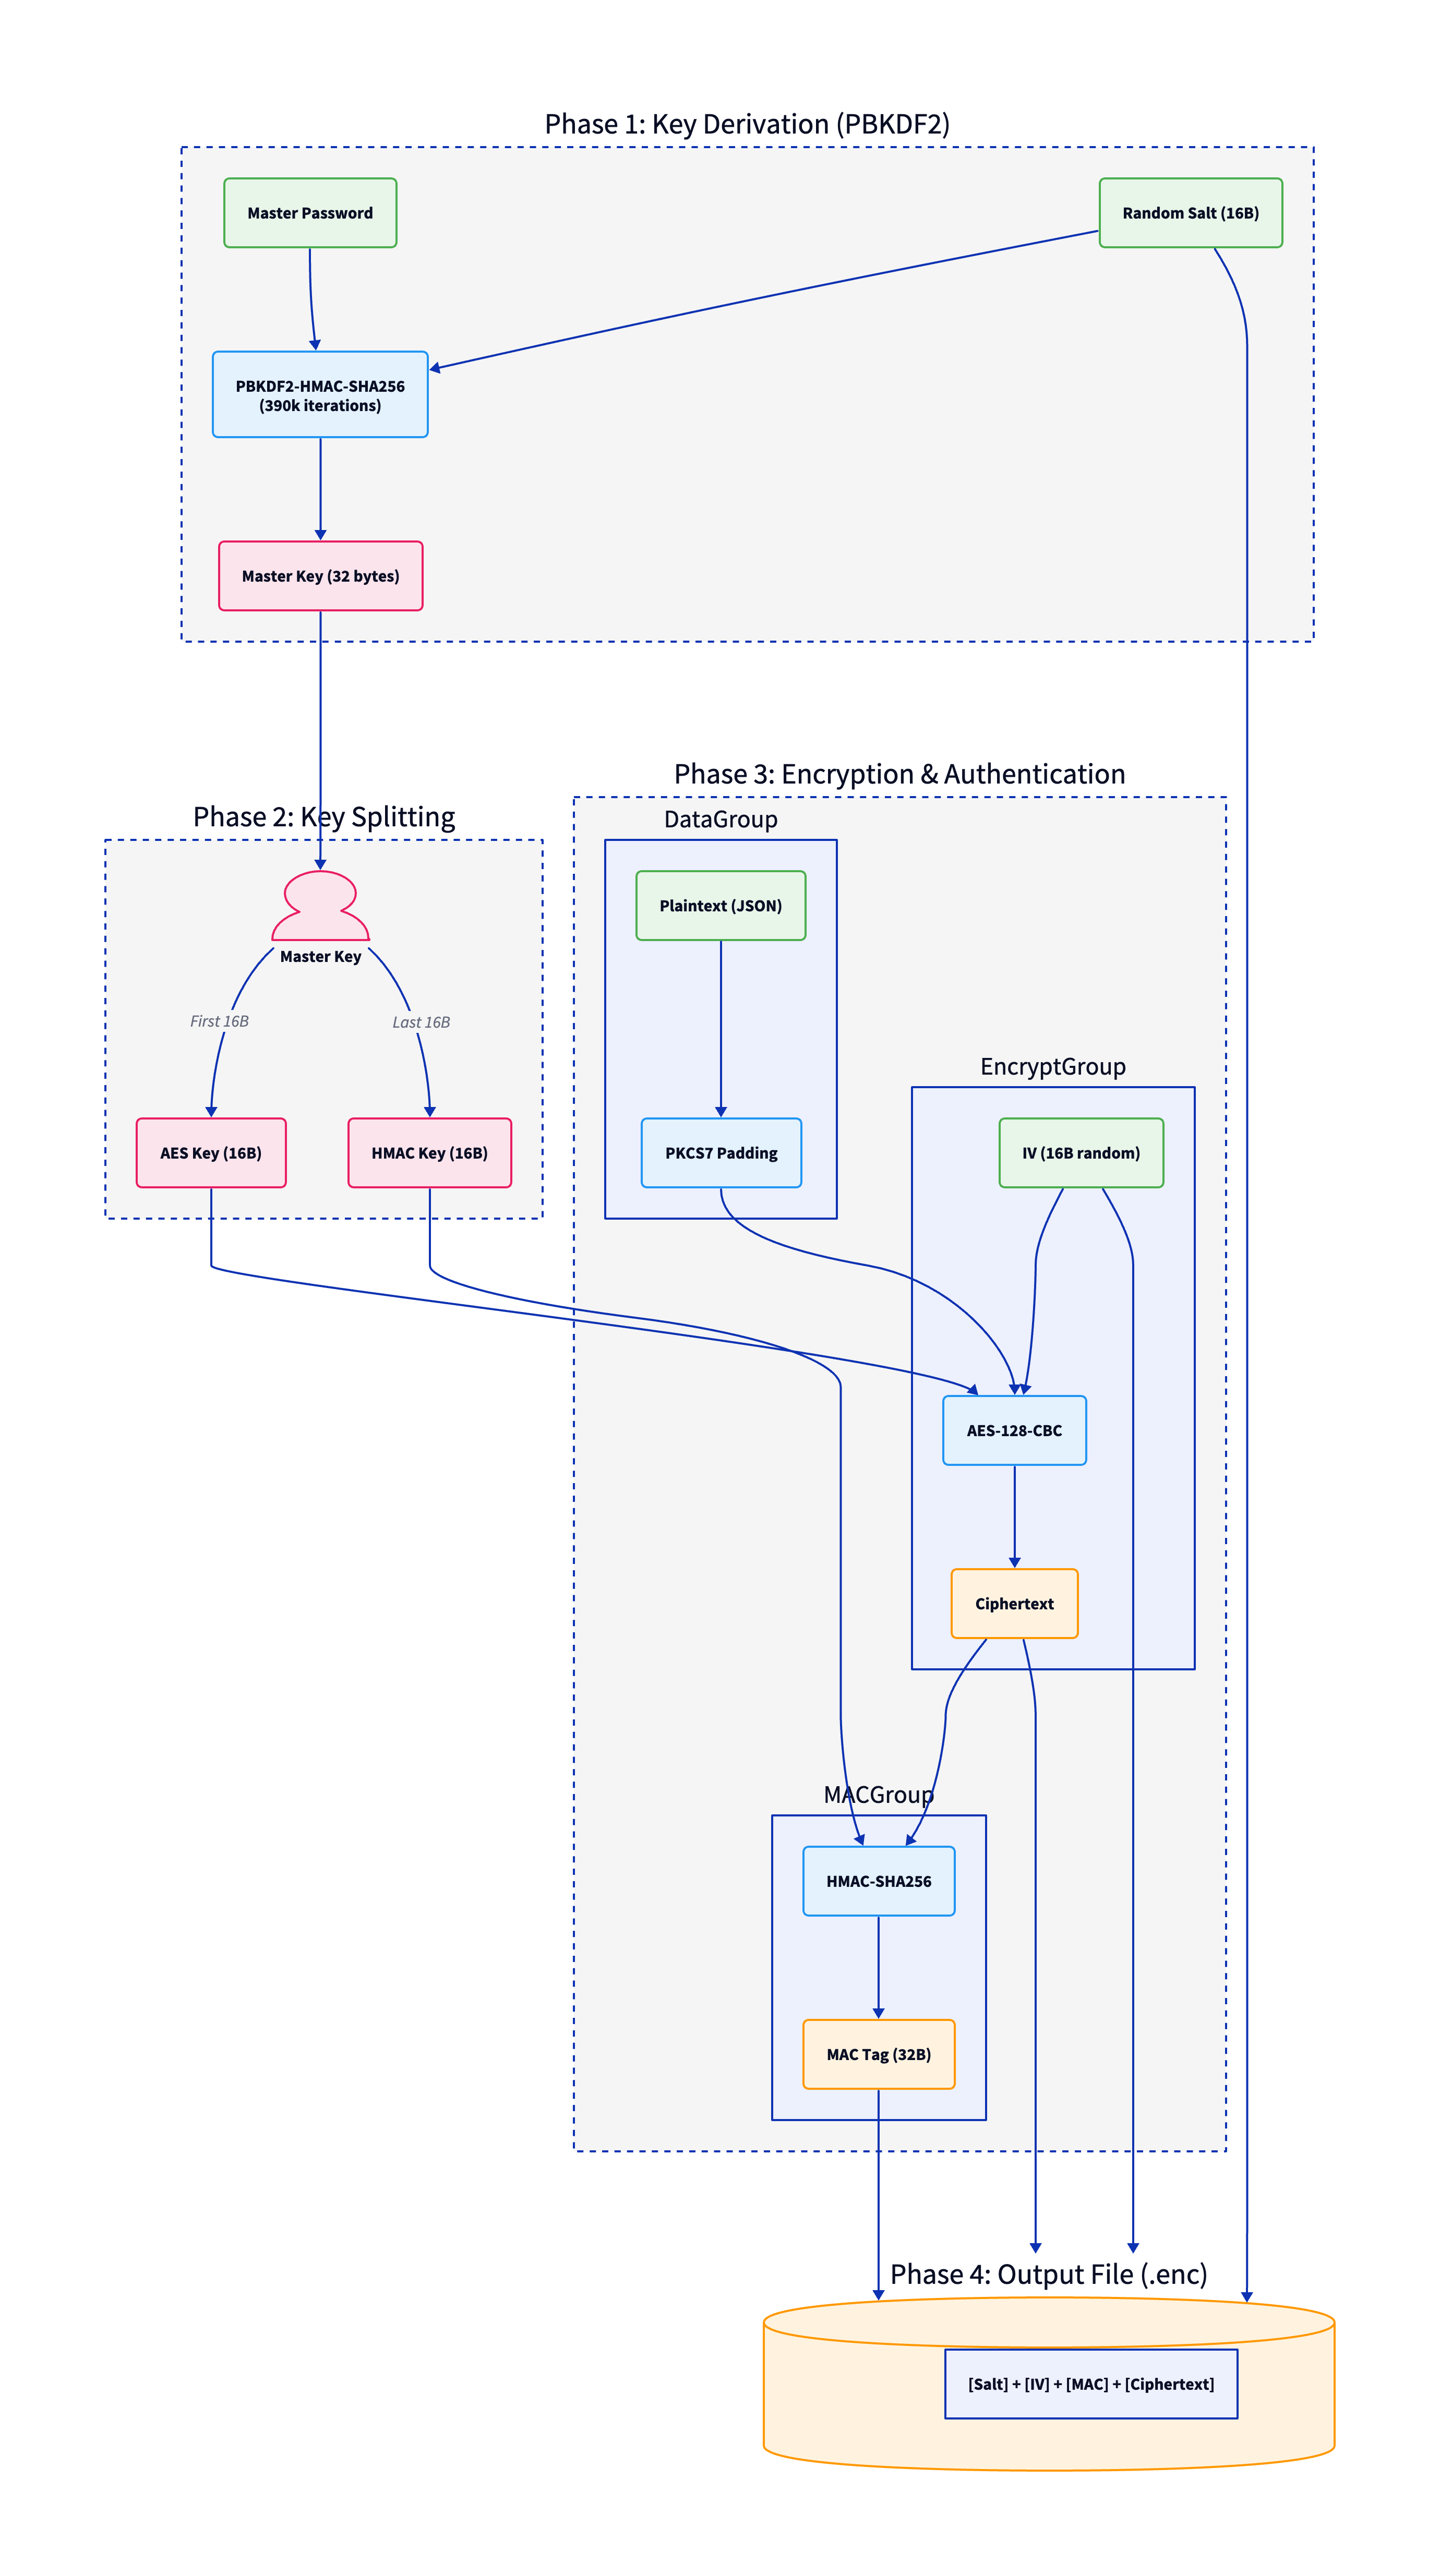
\includegraphics[width=0.8\textwidth]{../figure/figure_1a_encryption_flow.png}
    \caption{Phase-based Encryption Flow}
    \label{fig:enc_flow}
\end{figure}

\subsection{Vault File Specification}
The final encrypted output is a binary file organized as shown in Figure \ref{fig:file_format}. Each component (Salt, IV, MAC, and Ciphertext) has a fixed location to allow for reliable extraction during decryption.

\begin{figure}[h]
    \centering
    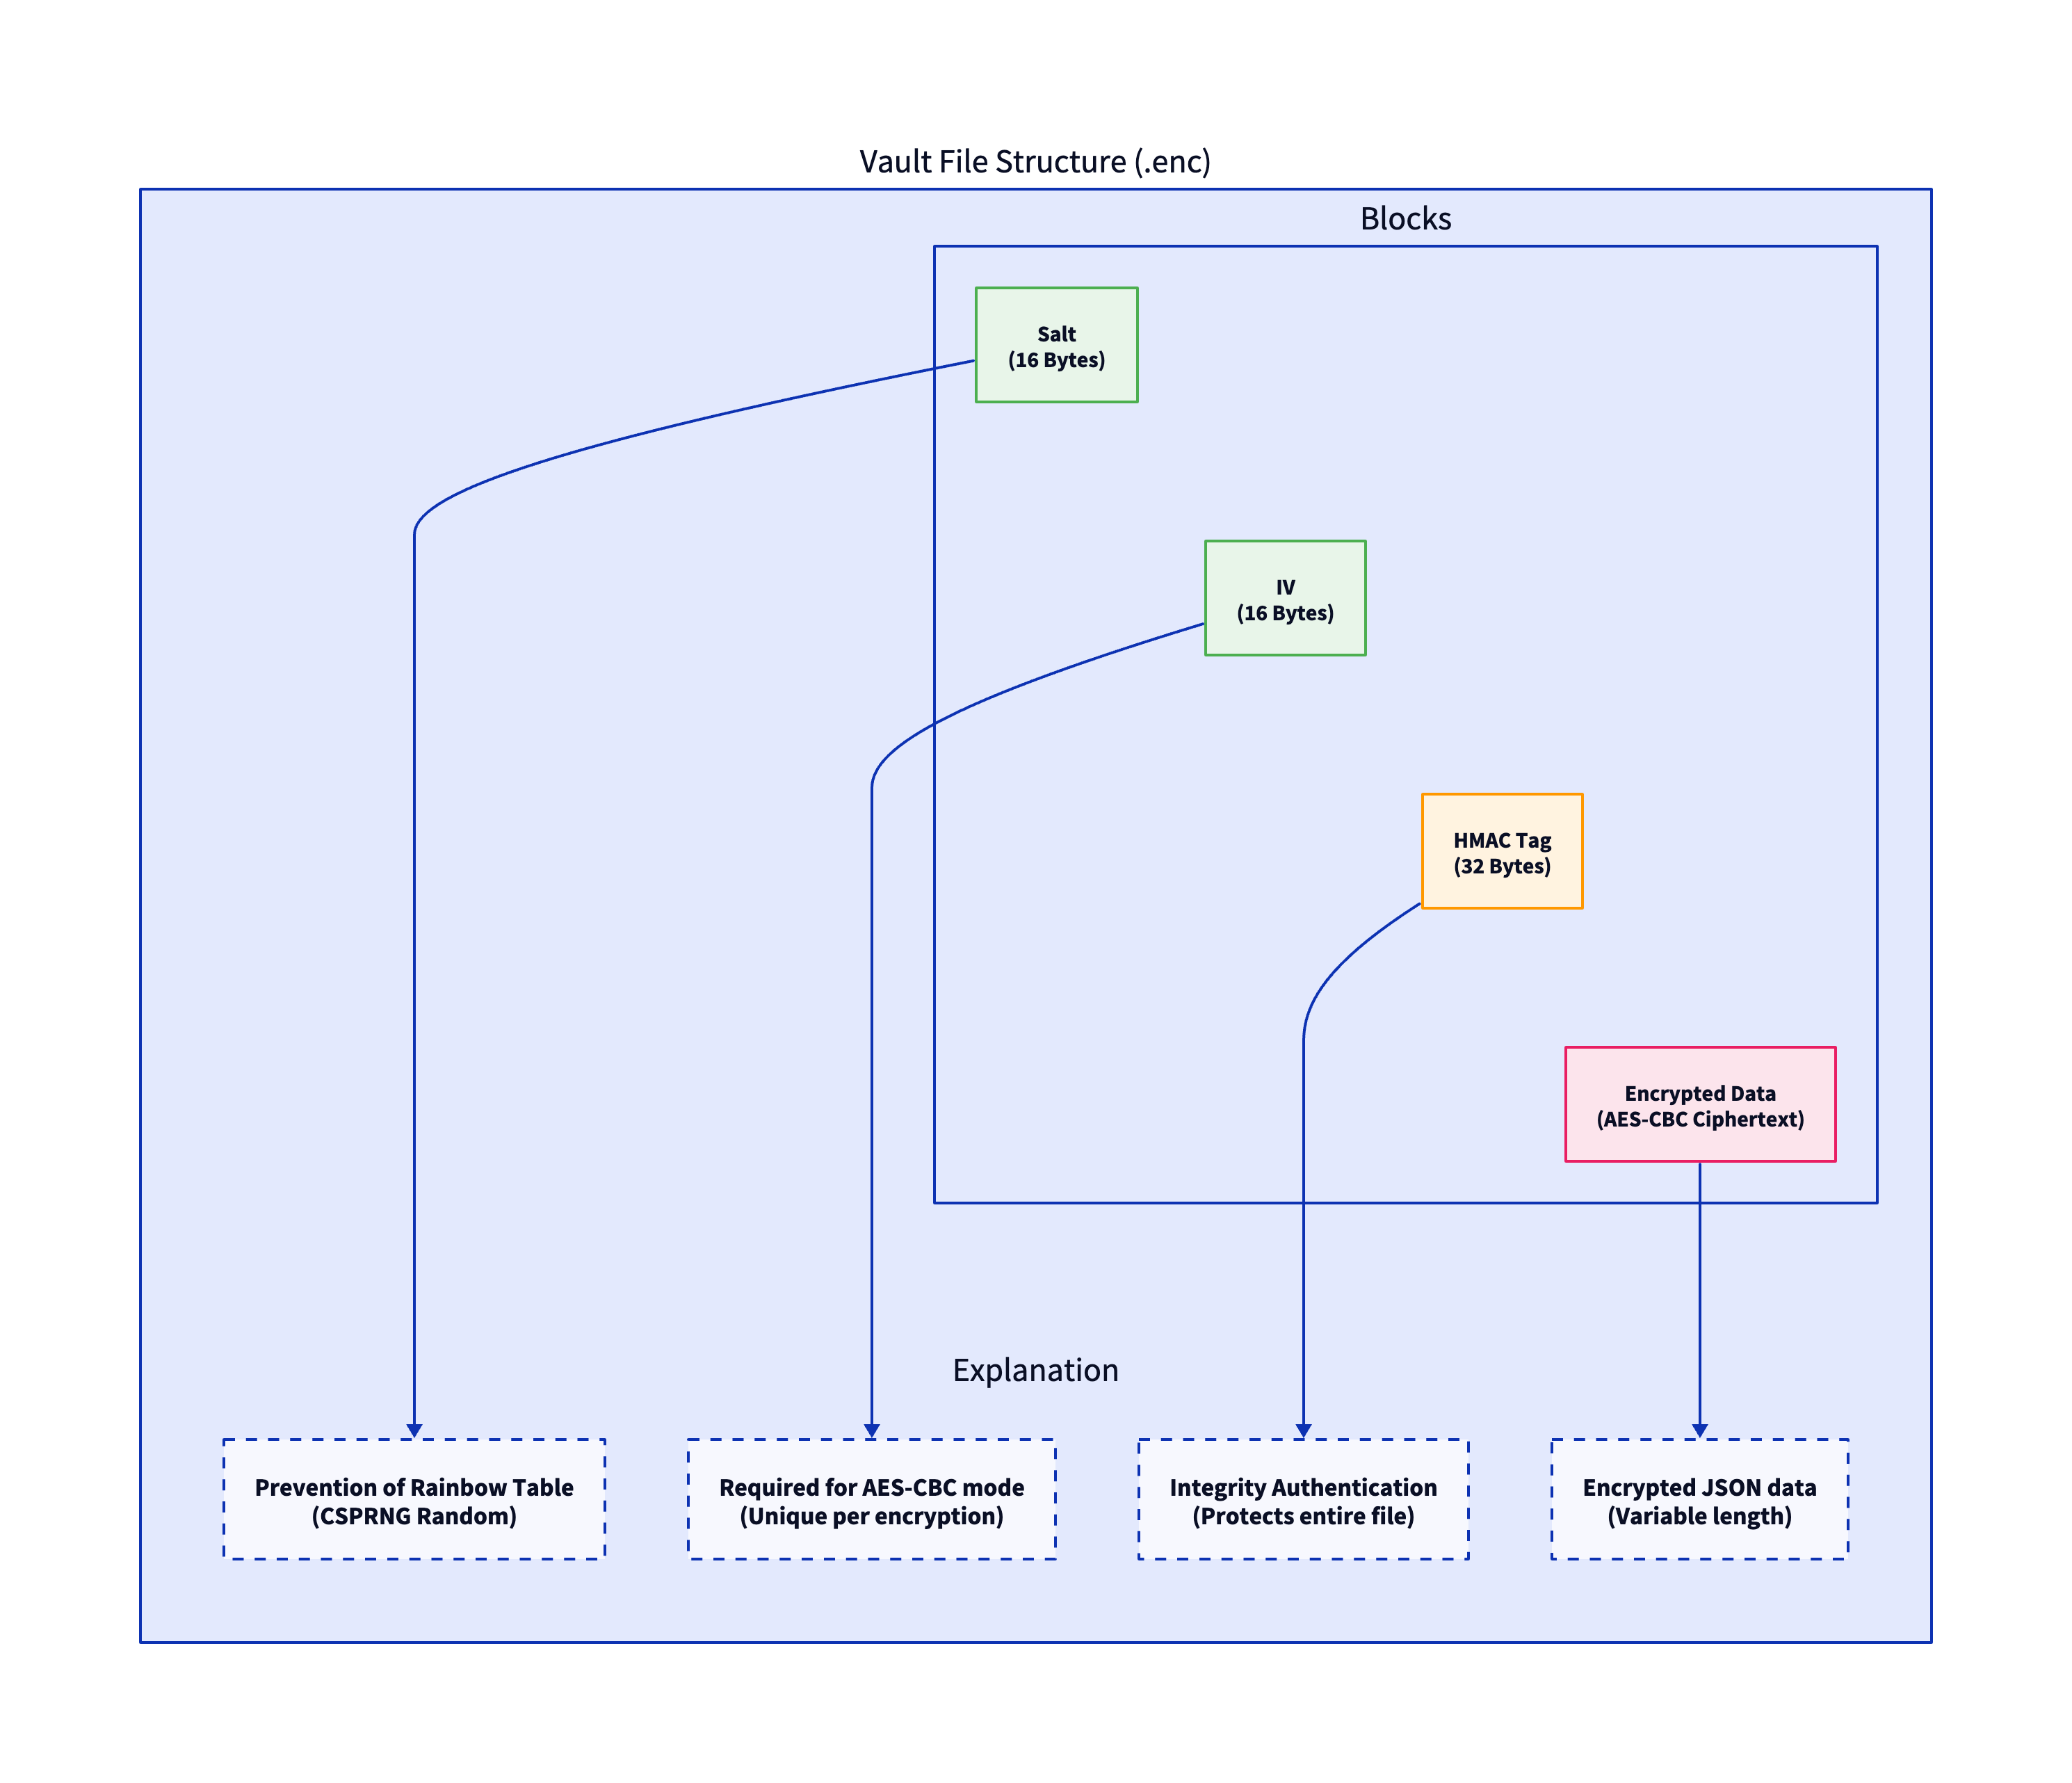
\includegraphics[width=0.8\textwidth]{../figure/figure_2_file_format.png}
    \caption{Encrypted Vault File Format}
    \label{fig:file_format}
\end{figure}
